\section{Ground Truth Generation: ArUco Board (Refined Approach)}
To overcome the limitations of the initial ellipse fitting 
approach, a second method was developed using ArUco board. This method aimed to achieve precise 3D estimation of the steering wheel's location and orientation. 
The use of ArUco board allowed for a more robust and accurate approach to capture the 3D 
geometry of the steering wheel. By leveraging the known 
properties and spatial relationships of the ArUco markers, 
this refined method was able to provide a reliable and 
high-quality ground truth for the steering wheel's position 
and orientation, which could then be used for training and 
evaluating 3D object detection models.

ArUco markers \cite{opencv_aruco_detection} are widely used  in 
computer vision for precise localization and pose estimation 
tasks.  An ArUco marker as depicted in \cref{fig:marker}, is a 
synthetic square marker featuring a  thick black border and an 
inner binary matrix that encodes  its identifier (ID). The black 
border enables quick detection  in images, while the binary 
matrix allows for identification  and supports error detection 
and correction.  The marker size dictates the dimensions of the 
internal matrix;  for example, a 4x4 marker contains 16 bits. They offer 
several advantages, including robustness to  variations in 
lighting, simple detection with minimal  computational overhead, 
and compatibility with popular  libraries like OpenCV \cite{opencv_library}, which 
provides dedicated functions for detecting ArUco markers and 
estimating their pose in both 2D  and 3D. Figures \cref{fig:marker_detection} and \cref{fig:marker_orientation} demonstrate OpenCV's capabilities in detecting ArUco markers and 
estimating their 3D position, respectively. 

\begin{figure}[htpb]
    \centering
    \begin{subfigure}[t]{0.3\textwidth}
        \centering
        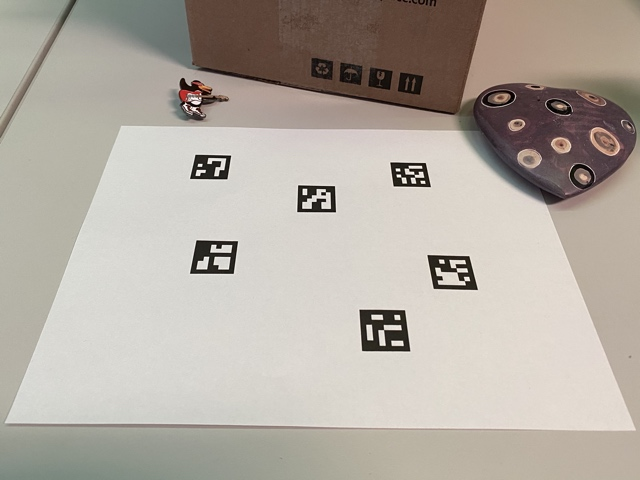
\includegraphics[width=\textwidth]{media/chapter 5/singlemarkersoriginal.jpg}
        \caption{Single ArUco Markers}
        \label{fig:marker}
    \end{subfigure}\hfill
    \begin{subfigure}[t]{0.3\textwidth}
        \centering
        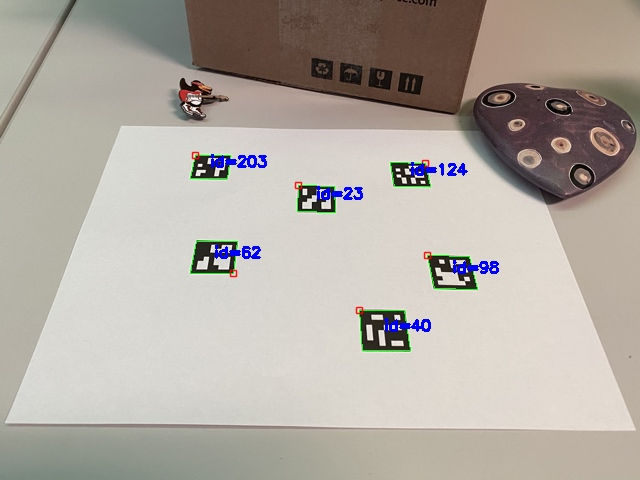
\includegraphics[width=\textwidth]{media/chapter 5/singlemarkersdetection.jpg}
        \caption{These are the detected markers (in green). 
        Note that some markers are rotated. 
        The small red square indicates the marker’s top left 
        corner}
        \label{fig:marker_detection}
    \end{subfigure}\hfill
    \begin{subfigure}[t]{0.3\textwidth}
        \centering
        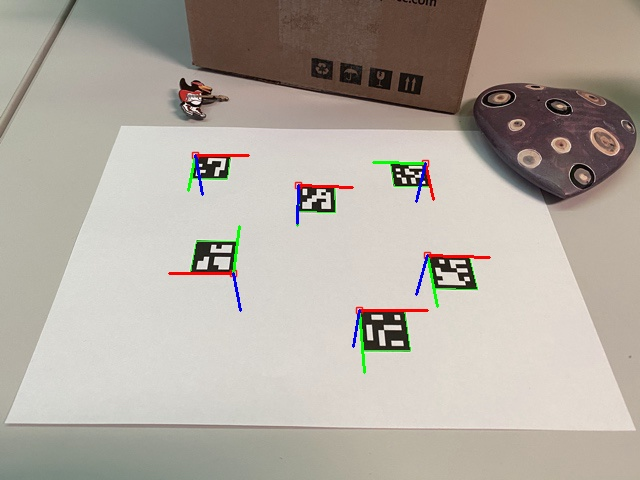
\includegraphics[width=\textwidth]{media/chapter 5/singlemarkersaxes.jpg}
        \caption{The marker coordinate system that is placed in the center or in the top left 
        corner of the marker with the Z axis pointing out. 
        Axis-color correspondences are X: red, Y: green, Z: blue.}
        \label{fig:marker_orientation}
    \end{subfigure}
    \caption{ArUco markers detection and pose estimation by OpenCV.}
\end{figure}

This refined approach aimed to address the challenges 
encountered in the initial method, particularly the issues of 
data sparsity, noise, and inaccurate geometric representation. 
By leveraging the advantages of ArUco board, this method 
sought to tackle the difficulties in precisely estimating the 
3D location and orientation of the steering wheel. 

The proposed technique involved positioning a board with 
multiple ArUco markers at the center of the steering wheel 
like in \cref{fig:gt_stream} and fitting a plane to the ArUco board to 
enhance the accuracy of orientation estimation. 
This setup allowed us to capture both the 2D and 3D spatial data required for accurately estimating the steering wheel's position.

The methodology involved two primary components for estimating 
the location and orientation of the steering wheel. 
each component is described in detail in the following 
sections:

\subsection{Location Estimation}
As depicted in \cref{fig:gt_stream}, the ArUco board is positioned at the center of the steering 
wheel. Therefore, the detected centroid of the ArUco board directly 
corresponds to the 3D spatial coordinates of the steering 
wheel's center. Given the known arrangement of markers on the 
ArUco board, the location of the board's center, and 
consequently the steering wheel's center, can be readily 
inferred from the detected positions of the individual markers.
To achieve precise location estimation of the ArUco markers, two primary approaches are considered:

\textbf{1. Direct 3D Estimation Using OpenCV: }
OpenCV’s \emph{estimatePoseSingleMarkers} function provides a direct 
way to estimate the 3D position of markers relative to the camera. 
This function relies on the known physical size of the 
ArUco markers and the intrinsic camera parameters to calculate 
the translation vector, which represents the 3D position of 
the markers as [dx, dy, dz] where dx dy, and dz are the marker's 
position along the x, y, and z axes, respectively. 
While this method offers a straightforward approach, its 
accuracy can be sensitive to markers' orientation, distance from 
the camera, and the angle of view.


\textbf{2. 2D Estimation with Mapping to 3D: }
This alternative method starts by detecting the 2D position of 
the markers in the image plane using OpenCV’s \emph{detectMarkers} 
function. \Cref{fig:detectMarkers} shows markers' location detected 
by OpenCV on the 2D image.
After detecting the 2D positions, these points are 
mapped to 3D space using depth information derived from the 
point cloud data and the camera’s intrinsic parameters. 
This approach separates the detection process into two stages, 
potentially improving accuracy by isolating the detection of 
2D marker positions from their 3D mapping.
\begin{figure}[htpb]
    \centering
    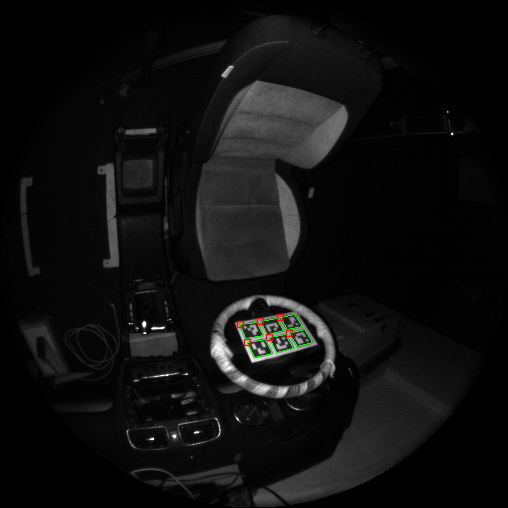
\includegraphics[width=0.5\textwidth]{media/chapter 5/aruco_detection.png}
    \caption{OpenCV detected the ArUco markers' location in the 2d image.}
    \label{fig:detectMarkers}
\end{figure}


Given the known structure and location of individual markers on 
the board, from each of the above approaches, 
we employed a method to calculate the board’s center based on the 
spatial relationship of specific marker pairs. This technique ensured 
that the center could be reliably calculated even if some markers were 
undetected.

To calculate the center of the board, three pairs of markers are utilized 
that are symmetrically positioned on opposite sides of the board. As depicted
in \cref{fig:marker_ids}. these marker pairs are \{(0, 5), (1, 4), (2, 3)\}
for a 2x3 board. 
For each detected pair, the midpoint between the two markers was 
computed by averaging their translation vectors \( tvec \), which 
represent the 3D coordinates of each marker. This midpoint provides an 
estimate of the board’s center based on that particular pair.
For each detected pair \((i, j)\), the midpoint is computed as:
\[
{midpoint}_{ij} = \frac{tvec_i + tvec_j}{2}
\]

where  \(tvec_i\)  and  \(tvec_j\)  are the translation vectors 
(3D coordinates) of markers  \(i\)  and  \(j\) . Once the midpoints for 
all detected pairs are obtained, the overall center of the board is 
calculated as the mean of these midpoints:

\[
{center}_{board} = \frac{\sum_{(i, j) \in {detected pairs}} {midpoint}_{ij}}{N}
\]

where  \(N\)  is the number of detected pairs. The resulting averaged 
translation vector represents the estimated 3D center of the board. 


By considering the relative positions and midpoints of detected marker 
pairs, this method can robustly determine the center point of the board despite the potential occlusions or missing markers.

\begin{figure}[htpb]
    \centering
    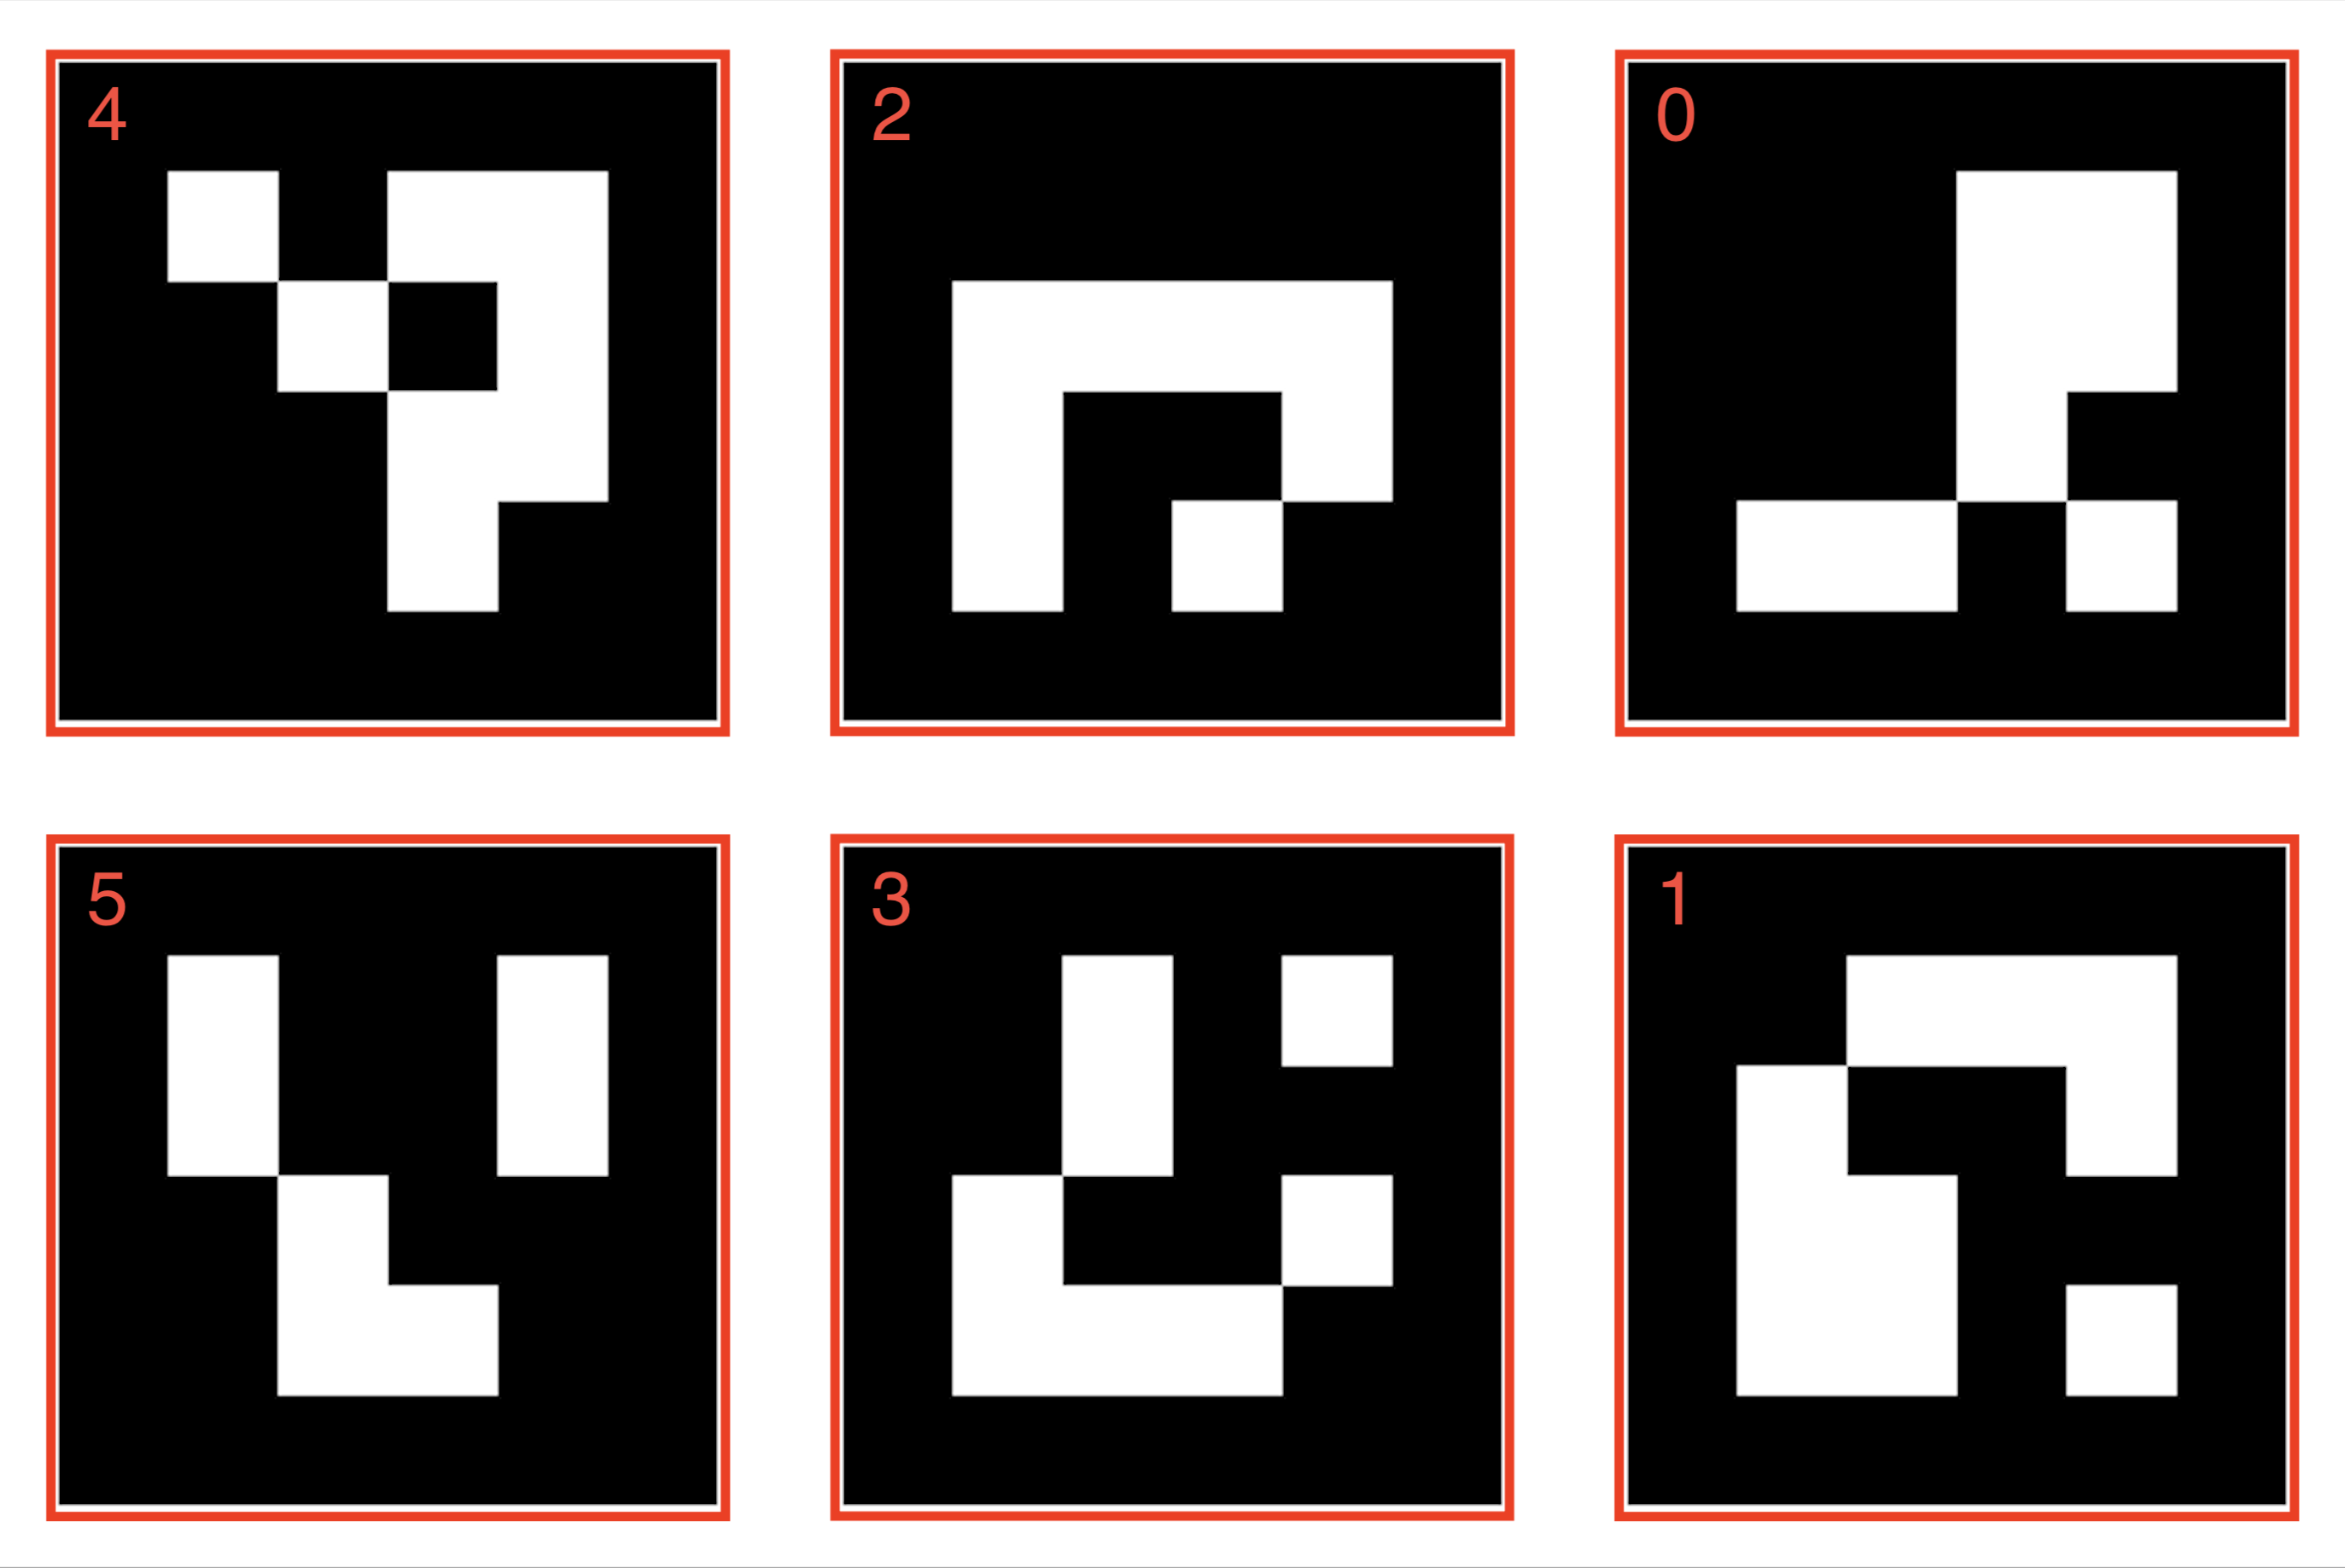
\includegraphics[width=0.5\textwidth]{media/chapter 5/aruco_board_ids.png}
    \caption{To calculate the center of the board, multiple 
    marker pairs are considered that are symmetrically positioned on opposite sides of the board as marker pairs \{(0,5), (1,4), (2,3)\} for a 2x3 board.}
    \label{fig:marker_ids}
\end{figure}


\subsection{Orientation Estimation}
Accurately determining the orientation of the marker board was 
critical for estimating the steering wheel’s orientation. 
As the ArUco board is accurately placed tangent to the steering 
wheel, the orientation of the board corresponds to the 
orientation of the steering wheel in 3D space. 
Two methods were exploited to estimate the orientation of 
the ArUco board: 

\textbf{1. Direct Orientation Estimation Using OpenCV: }
OpenCV’s \emph{estimatePoseSingleMarkers} function also calculates the 
orientation of markers in the form of rotation vectors. 
These vectors indicate the rotational pose of each marker 
relative to the camera’s coordinate system. Assuming that orientation of the markers on the board are known, the overall orientation of the board
can be estimated by removing the outlier rotation vectors and averaging the remaining. However, this method has limitations, as it relies on the 
accuracy of OpenCV's built-in pose estimation.

As illustrated in \cref{fig:estimatePoseSingleMarkers}, 
OpenCV's estimations of markers' orientation on a 3×4 board are highly sensitive to several factors. 
These include the camera angle, the distance of the markers from 
the camera, occlusion of the markers, and other environmental 
factors. Consequently, when markers are missing or occluded, 
the reliability and accuracy of the orientation estimation can 
decrease significantly. This sensitivity to various spatial and 
environmental conditions highlights the limitations of relying 
solely on OpenCV's built-in pose estimation functions for robust 
3D orientation determination.

\begin{figure}[htpb]
    \centering
    \begin{subfigure}[t]{0.23\textwidth}
        \centering
        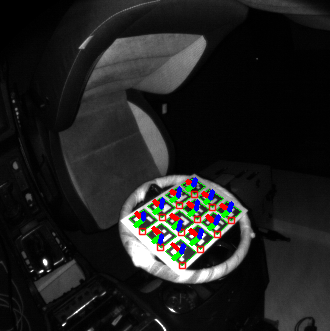
\includegraphics[width=\textwidth]{media/chapter 5/aruco_board_estimation0.png}
    \end{subfigure}\hfill
    \begin{subfigure}[t]{0.23\textwidth}
        \centering
        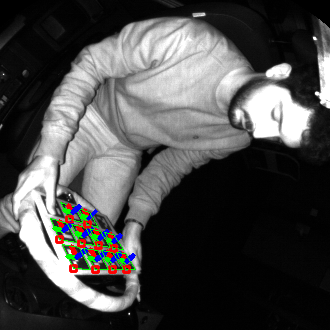
\includegraphics[width=\textwidth]{media/chapter 5/aruco_board_estimation1.png}
    \end{subfigure}\hfill
    \begin{subfigure}[t]{0.23\textwidth}
        \centering
        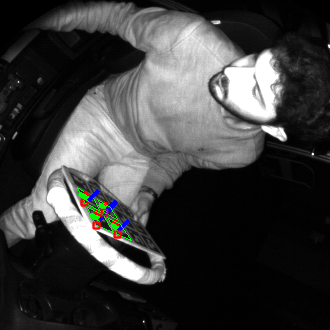
\includegraphics[width=\textwidth]{media/chapter 5/aruco_board_estimation2.png}
    \end{subfigure}\hfill
    \begin{subfigure}[t]{0.23\textwidth}
        \centering
        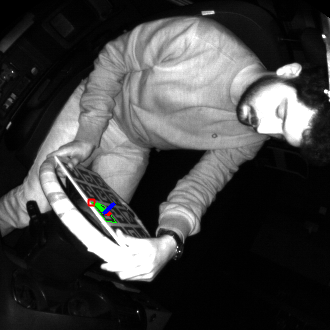
\includegraphics[width=\textwidth]{media/chapter 5/aruco_board_estimation3.png}
    \end{subfigure}
    \caption{The markers' coordinate system estimated by OpenCV's
            \emph{estimatePoseSingleMarkers} function on a 3x4
            board shows that this method is highly sensitive
            to the markers' distance, camera angle and other
            environmental factors. Axis-color correspondences are 
            X: red, Y: green, Z: blue, with Z axis pointing out}
    \label{fig:estimatePoseSingleMarkers}
\end{figure}

\textbf{2. Plane Fitting Method: }
The plane fitting method provided a more robust and reliable 
means of estimating the orientation, as it doesn't depend solely 
on the accuracy of OpenCV's pose estimation for individual 
markers. This approach overcomes the limitations of the direct 
orientation estimation using OpenCV, which can be sensitive to 
factors like marker size, distance, and viewing angle. 
Hence, the plane fitting method offers a more stable and 
accurate estimate of the steering wheel's orientation under a 
variety of conditions.
This method involves the following steps:

\begin{enumerate}
    \item \emph{Finding Center of the ArUco Board: }
    To initiate plane fitting, it is essential to first locate 
    the center of the ArUco board. This is done using the 
    detected marker locations. Given that the markers are 
    arranged in a known, fixed structure on the board, 
    the center can be reliably estimated even if one or more 
    markers are not detected.
    \item \emph{Sampling Points Around the Center: }
    Once center of the ArUco board is determined, 
    a set of points are sampled from the board around this 
    central point within a specified radius. This sampling 
    process ensures that the points used for plane fitting are 
    well-distributed across the board, enhancing the reliability 
    of the orientation estimation. \Cref{fig:plane_fitting} shows 
    the sampled points from the board in red.
    \item \emph{Fitting a Plane to the Sampled Points: }
    The sampled points are then used to fit a plane. 
    The fitting process involves computing the best-fit plane 
    that minimizes the distance between the plane and the 
    sampled points. This plane effectively represents the 
    overall orientation of the ArUco board.
    \item \emph{Using the Normal Vector for Orientation: }
    The normal vector of the fitted plane is then calculated. 
    This normal vector serves as a robust indicator of 
    the board’s orientation in 3D space. As \cref{fig:plane_fitting}
    shows, the light blue line indicated the norm vector of the board.
    Since the board is mounted on the steering wheel tangent to the 
    steering wheel's surface, the orientation of this normal vector 
    directly corresponds to the orientation of the steering wheel.
\end{enumerate}

\begin{figure}[htpb]
    \centering
    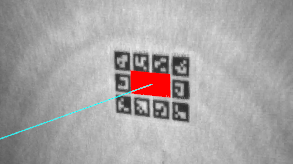
\includegraphics[width=0.5\textwidth]{media/chapter 5/plane_fitting.png}
    \caption{Illustration of the plane fitting method, showing the 
    sampled points around the center of a 3x4 ArUco board in red and the 
    normal vector of the fitted plane in light blue, which represents 
    the orientation of the ArUco board.}
    \label{fig:plane_fitting}
\end{figure}

One of the significant advantages of this method is its 
robustness to marker detection failures. Even if some markers 
are not detected due to occlusions, lighting conditions, or 
other factors, it doesn't affect the plane fitting approach's accuracy. This makes the plane fitting method highly 
resilient to errors in individual marker detections, ensuring 
reliable orientation estimation under a variety of conditions.



\section{Evaluation}
The evaluation phase was designed to rigorously assess the accuracy 
and reliability of the methods employed for both location and 
orientation estimation of the ArUco board and, by extension, the 
steering wheel. For this purpose, two experiments are conducted:
\begin{itemize}
    \item \textbf{Inter-Marker Distance Evaluation}, which focused on the 
    accuracy of the location estimation methods.
    \item \textbf{Distance and Angle Variation}, which tested the robustness 
    of both location and orientation estimation methods under varying 
    spatial conditions.
\end{itemize}

Through these experiments, the evaluation sought to provide a 
comprehensive analysis of the methods, highlighting their strengths 
and limitations.

\subsection{Experiment 1: Inter-Marker Distance Evaluation}
To assess the accuracy of the location estimation methods, a marker board with known geometric properties was used. The actual distances between the markers on the board were predefined and served as the ground truth. The dimensions provided in \cref{fig:marker_dimention} were used to calculate the distances between the markers, as well as the distances between the markers and center of the board. \Cref{fig:distance_matrix} depicts the distance matrix of the 3x4 ArUco board used for this experiment.

\begin{figure}[htpb]
    \centering
    \includegraphics[width=0.5\textwidth]{media/chapter 5/board_geometry.png}
    \caption{Geometry of the 3x4 ArUco board used in the experiment 1. Distances between markers and the center of the board can be calculated using the dimensions provided in the figure.}
    \label{fig:marker_dimention}
\end{figure}

\begin{figure}[htpb]
    \centering
    \includegraphics[width=0.9\textwidth]{media/chapter 5/Distance Matrix.png}
    \caption{Distance matrix of the markers and center of the board for the 3x4 ArUco board used in experiment 1.}
    \label{fig:distance_matrix}
\end{figure}

Both the OpenCV's direct 3D estimation and the 2D estimation with mapping to 3D methods were used to estimate the 3D location of the markers. The mean error of the calculated distances between the markers was then computed to evaluate each location estimation method.

\subsection{Experiment 2: Distance and Angle Variation}
The second experiment tested the robustness of the location and orientation estimation methods under varying conditions. The marker board was placed on a wall and the camera placed at different distances of  90, 95, 100, 105, and 110 cm from the board and titled downward and upward with angles of -15°, -10°, -5°, 0°, 5°, 10°, and 15° relative to the horizon. \Cref{fig:board_on_wall_plain_fitting} illustrates the experiment setup with camera placed at 100 cm far from the board and tilted 0° downward. 

\begin{figure}[htpb]
    \centering
    \begin{subfigure}[t]{0.45\textwidth}
        \centering
        \includegraphics[width=\textwidth]{media/chapter 5/board_on_the_wall.png}
        \caption{The red region represents the plane fitted to the board, with the light blue vector indicating the normal vector of this plane. The camera’s coordinate system is shown by the dark blue (z-axis), red (x-axis), and green (y-axis) vectors.}
        \label{fig:board_on_wall_plain_fitting}
    \end{subfigure}\hfill
    \begin{subfigure}[t]{0.45\textwidth}
        \centering
        \includegraphics[width=\textwidth]{media/chapter 5/aruco_board_on_the_wall.png}
        \caption{Markers' orientation estimated by OpenCV. color codes are as: dark blue (z-axis), red (x-axis), and green (y-axis)}
        \label{fig:board_on_wall_opencv}
    \end{subfigure}
    \caption{Experimental setup for steering wheel position estimation. The camera is positioned 100 cm away from the ArUco board, facing straightforward.}
\end{figure}

This experiment was designed to evaluate how well each method maintained accuracy across different spatial configurations, simulating real-world conditions where the camera's position and angle can change relative to the steering wheel. The experiment aimed to assess the performance of the location and orientation estimation methods discussed in section 5.2 under a range of realistic scenarios, with the marker board positioned at different distances and angles to mimic the potential variations in the camera's placement and orientation relative to the steering wheel in practical applications.

The accuracy of the location estimation methods was evaluated by comparing the estimated distances from the camera to the board with the actual distances. Additionally, the accuracy of the orientation estimation methods was assessed by comparing the estimated orientation with the ground truth orientation of the camera.

\section{Results}
The evaluation of the ArUco-board-based approach for steering wheel position and orientation estimation revealed clear distinctions in the performance of the tested methods. Through a series of experiments, both location and orientation estimation techniques were assessed to determine their accuracy, robustness, and reliability under varying spatial configurations.

This section presents the results from these experiments, covering both location estimation and orientation estimation outcomes. The findings are organized as follows:

\subsection{Locaiton Estimation}
The results from the two experiments demonstrated clear differences between the two methods:

\textbf{Inter-Marker Distance Evaluation:}
Both OpenCV’s direct 3D estimation method and the 2D-to-3D mapping approach were applied to estimate the 3D locations of the markers. The mean error in the calculated distances between markers is illustrated in \cref{fig:distance_error_matrix}, showing that the 2D-to-3D mapping method consistently outperformed direct 3D estimation, achieving significantly lower mean errors and deviations in the estimated distances between markers.

\Cref{tab:mse} provides a detailed comparison of the mean squared error (MSE) in the inter-marker distances for each location estimation method. Additionally, it includes the estimated distance between the marker board and the camera, with the board positioned at the actual distance of 72.9 cm. The results show that the 2D-to-3D mapping approach provides a more precise estimate of both the inter-marker distances and the overall board-to-camera distance compared to the direct 3D estimation.

Overall, this experiment demonstrated the clear advantage of the 2D-to-3D mapping approach, which consistently delivered lower mean errors in the inter-marker distances. This suggests that the 2D-to-3D mapping method captured the true spatial relationships between markers more effectively, while the direct 3D estimation was more prone to inaccuracies and distortions. The superior accuracy of the 2D mapping approach highlights its robustness and reliability, making it an excellent choice for precise location estimation in steering wheel detection tasks.

\begin{figure}[htpb]
    \centering
    \begin{subfigure}[t]{0.65\textwidth}
        \centering
        \includegraphics[width=\textwidth]{media/chapter 5/opencv_error_matrix.jpg}
        \caption{}
    \end{subfigure}\\
    \begin{subfigure}[t]{0.65\textwidth}
        \centering
        \includegraphics[width=\textwidth]{media/chapter 5/point_cloud_error_matrix.jpg}
        \caption{}
    \end{subfigure}
    \caption{Inter-marker distance matrix errors for direct 3D estimation (a) and 2D mapping approaches (b) on a 3x4 ArUco board.}
    \label{fig:distance_error_matrix}
\end{figure}

\begin{table}[htpb]
    \caption{Inter-marker distance Mean Square Erorr for both locaiton estimation approaches.}
    \label{tab:mse}
    \centering
    \begin{tabular}{ l | p{0.25\textwidth} p{0.25\textwidth} |}
        \cline{2-3}
        & \multicolumn{1}{|p{0.25\textwidth}}{\centering direct 3D estimation using openCV} &  \multicolumn{1}{p{0.25\textwidth}|}{ \centering 2D estimation with mapping to 3D} \\
        \hline
        \multicolumn{1}{|l|}{inter-marker distance MSE} &  \multicolumn{1}{|p{0.25\textwidth}}{\centering 2.28} &  \multicolumn{1}{p{0.25\textwidth}|}{ \centering 0.42}\\
        \multicolumn{1}{|l|}{estimated board distance with the camera} &  \multicolumn{1}{|p{0.25\textwidth}}{\centering 78.33 cm} &  \multicolumn{1}{p{0.25\textwidth}|}{\centering 73.12 cm}\\
        \cline{2-3}
        \multicolumn{1}{|l|}{actual board distance with the camera} & \multicolumn{2}{c|}{\centering 72.9 cm}\\
        \hline
    \end{tabular}
\end{table}

\textbf{Distance and Angle Variation: }
\Cref{fig:opencv_distance_mean_error} and \Cref{fig:2d_mapping_distanc_mean_error} show the board’s distance mean error over all tested experiment setups. comparing the mean errors in different distance and angle configurations revealed that the direct 3D estimation method struggled to maintain accuracy as the distance and angle between the camera and the marker board increased. On the other hand, the 2D mapping approach coupled with the plane fitting method demonstrated superior performance, maintaining consistently high accuracy across the range of distances and angles tested. 


On the other hand, as illustrated in \cref{fig:opencv_distances} and \cref{fig:2d_mapping_distances}, the direct 3D estimation approach exhibited significantly greater deviations in the location estimation results across the full range of tested distance and angle configurations. This indicates that the direct 3D estimation method struggled to maintain consistent accuracy as the spatial relationship between the camera and marker board changed. Meanwhile, the 2D mapping approach demonstrated remarkably low deviations in the location estimation results, even under the varying distance and angle conditions.

The results of the distance and angle variation tests highlight a clear advantage of the 2D mapping approach over the direct 3D estimation method. As distance and angle increased, the direct 3D estimation method exhibited significant accuracy loss and high deviations, indicating its sensitivity to changes in spatial configuration. In contrast, the 2D mapping approach maintained consistently low mean errors and deviations, proving resilient across all tested conditions. This robustness underscores the reliability of the 2D mapping method for precise location estimation in variable settings, making it well-suited for accurate steering wheel’s location estimation in practical applications.

\begin{figure}[htpb]
    \centering
    \begin{subfigure}[t]{0.45\textwidth}
        \centering
        \includegraphics[width=\textwidth]{media/chapter 5/board's distance by opencv.png}
        \caption{Board's distance mean errors estimated by OpenCV in different experiment setups.}
        \label{fig:opencv_distance_mean_error}
    \end{subfigure}\hfill
    \begin{subfigure}[t]{0.45\textwidth}
        \centering
        \includegraphics[width=\textwidth]{media/chapter 5/board’s distance mean error estimated by mapping from 2D to 3D.png}
        \caption{Board's distance mean errors estimated by mapping from 2D to 3D in different experiment setups.}
        \label{fig:2d_mapping_distanc_mean_error}
    \end{subfigure}\\
    \begin{subfigure}[t]{0.45\textwidth}
        \centering
        \includegraphics[width=\textwidth]{media/chapter 5/board’s distances estimated by OpenCV.png}
        \caption{Board's distances estimated by OpenCV in 5 selected experiment setups.}
        \label{fig:opencv_distances}
    \end{subfigure}\hfill
    \begin{subfigure}[t]{0.45\textwidth}
        \centering
        \includegraphics[width=\textwidth]{media/chapter 5/board’s distances.png}
        \caption{Board's distances estimated by mapping from 2D to 3D in 5 selected experiment setups.}
        \label{fig:2d_mapping_distances}
    \end{subfigure}
    \caption{Comparing board's distance mean errors and distances in different experiment setups estimated by two location estimation approaches.}
    \label{fig:distance_error_matrix}
\end{figure}


\subsection{Orientation Estimation Results}
The orientation evaluation results further highlighted the clear advantages and superior performance of the plane fitting method for estimating the orientation of the marker board.

As \cref{fig:opencv_mean_angle} and \cref{fig:plane_fitting_mean_angle} illustrate, the plane fitting approach achieved significantly higher accuracy in estimating the marker board's orientation, as measured by the board’s angle with Z axis, compared to the direct estimation method using OpenCV's estimatePoseSingleMarker function. 

Additionally, direct orientation estimation with OpenCV shows significant higher variation compared with the plane fitting approach, as demonstrated by the standard deviation values in \cref{fig:opencv_angles} and \cref{fig:plane_fitting_angles}. 

These results demonstrate that the plane fitting method is not only more accurate in estimating the orientation, but also more robust and consistent in maintaining its performance under varying distance and angle conditions.
\begin{figure}[htpb]
    \centering
    \begin{subfigure}[t]{0.45\textwidth}
        \centering
        \includegraphics[width=\textwidth]{media/chapter 5/board’s mean angle with Z axis estimated by OpenCV.png}
        \caption{Board's mean angle with the camera's Z axis estimated by OpenCV in different experiment setups.}
        \label{fig:opencv_mean_angle}
    \end{subfigure}\hfill
    \begin{subfigure}[t]{0.45\textwidth}
        \centering
        \includegraphics[width=\textwidth]{media/chapter 5/board’s_ mean_angle_with_Z_axis_estimated_by_plane_fitting.png}
        \caption{Board's mean angle with the Z axis estimated by plane fitting in different experiment setups.}
        \label{fig:plane_fitting_mean_angle}
    \end{subfigure}\\
    \begin{subfigure}[t]{0.45\textwidth}
        \centering
        \includegraphics[width=\textwidth]{media/chapter 5/board’s angles with the camera Z axis estimated by OpenCV.png}
        \caption{Board's angles with the Z axis, estimated by OpenCV in 5 selected experiment setups.}
        \label{fig:opencv_angles}
    \end{subfigure}\hfill
    \begin{subfigure}[t]{0.45\textwidth}
        \centering
        \includegraphics[width=\textwidth]{media/chapter 5/board’s angles with camera's Z axis estimated by plane fitting.png}
        \caption{Board's angles with the Z axis, estimated by plane fitting in 5 selected experiment setups.}
        \label{fig:plane_fitting_angles}
    \end{subfigure}
    \caption{Comparing board's angles and mean angle with the Z axis in different experiment setups estimated by two rotation estimation approaches.}
    \label{fig:distance_error_matrix}
\end{figure}


\subsection{Systematic Error in Orientation Estimation}
A systematic error was identified in the camera’s coordinate system, with tilts of -1.28°, -6.13°, and -6.35° along the x, y, and z axes, respectively. This misalignment was corrected in subsequent estimations to ensure accuracy in the orientation calculations.
\Cref{fig:board_on_wall_plain_fitting} illustrates this deviation. Although the camera angle is 0, the orientation of the camera’s coordinate system shows a noticeable tilt, indicating the existence of a systematic error in the camera coordinate system.


\section{Conclusion}
In conclusion, this study presents a robust and accurate approach to estimate the 3D position and orientation of a steering wheel using a combination of 2D-to-3D mapping and plane fitting techniques. 

2D-to-3D mapping shows much higher accuracy in estimating the board’s location compared to direct 3D estimation, particularly as the distance and angle between the camera and board increase. On the other hand, plane fitting approach delivers superior performance in estimating the board's orientation, with significantly higher accuracy and lower variation compared to the direct estimation method.

Hence, with a combination of the 2D-to-3D mapping for location estimation and the plane fitting approach for orientation estimation, this study demonstrates a reliable, robust, and precise solution for determining the 3D pose of a steering wheel in the context of autonomous driving and human-vehicle interaction applications. 